\begingroup\emergencystretch=3em
\section{Deskripsi Dataset}
\label{sec:dataset}

Dataset berasal dari kompetisi Kaggle Tugas Besar 2 IF3170 (\url{https://www.kaggle.com/competitions/T2-IF3170-2026-2027}) dan berisi catatan pemesanan sebuah penginapan. Setiap baris adalah satu pemesanan, yang dicirikan oleh tamu, masa menginap, kanal pemesanan, dan harga. Tersedia tiga berkas:
\begin{itemize}
	\item \texttt{train.csv}: 27.373 baris dan 19 kolom (kolom \texttt{id}, 17 fitur, dan target \texttt{is\_canceled});
	\item \texttt{test.csv}: 6.844 baris dan 18 kolom (tanpa target);
	\item \texttt{sample\_\allowbreak submission.csv}: contoh format \textit{submission} berisi kolom \texttt{id} dan \texttt{is\_canceled}.
\end{itemize}
Kolom \texttt{id} adalah pengenal unik pesanan dan bukan fitur. Kolom ini harus dibaca sebagai teks, karena sebagian nilainya hanya berisi angka atau menyerupai notasi ilmiah (misalnya \texttt{123e4567}) dan akan rusak jika dibaca sebagai angka. Target adalah \texttt{is\_canceled}, yang hanya ada pada data latih.

\subsection{Deskripsi Fitur}
\label{subsec:deskripsi-fitur}

Dari 17 fitur, 14 bertipe numerik dan 3 kategorikal. Fitur dikelompokkan menurut tipenya pada Tabel~\ref{tab:fitur}. Kolom hitungan bertipe desimal pada data karena memuat nilai kosong. Kolom ``Kosong'' menunjukkan persentase nilai hilang pada data latih. Fitur yang tidak tercantum tidak memiliki nilai hilang. IDR adalah mata uang Rupiah.

\begin{longtable}{p{3.8cm} p{2.1cm} p{5.6cm} c}
	\caption{Deskripsi fitur dataset}\label{tab:fitur}\\
	\toprule
	\textbf{Fitur} & \textbf{Tipe} & \textbf{Deskripsi} & \textbf{Kosong} \\
	\midrule
	\endfirsthead
	\toprule
	\textbf{Fitur} & \textbf{Tipe} & \textbf{Deskripsi} & \textbf{Kosong} \\
	\midrule
	\endhead
	\texttt{days\_\allowbreak before\_\allowbreak arrival} & Kontinu & Selisih hari antara tanggal pemesanan dan kedatangan (\textit{lead time}); rentang 0--448 & 4,10\% \\
	\texttt{nightly\_\allowbreak rate\_\allowbreak idr} & Kontinu & Harga rata-rata per kamar per malam (IDR); 0 berarti menginap gratis (\textit{complimentary}); maksimum sekitar 9,2 juta & 7,45\% \\
	\midrule
	\texttt{num\_adults} & Hitungan & Jumlah tamu dewasa & 2,96\% \\
	\texttt{num\_children} & Hitungan & Jumlah tamu anak & 11,09\% \\
	\texttt{weekend\_\allowbreak nights} & Hitungan & Jumlah malam akhir pekan (Sabtu atau Minggu) & -- \\
	\texttt{weekday\_\allowbreak nights} & Hitungan & Jumlah malam hari kerja (Senin sampai Jumat) & -- \\
	\texttt{prior\_\allowbreak cancellations} & Hitungan & Jumlah pemesanan sebelumnya yang dibatalkan & -- \\
	\texttt{prior\_\allowbreak completed\_\allowbreak bookings} & Hitungan & Jumlah pemesanan sebelumnya yang tidak dibatalkan & -- \\
	\texttt{special\_\allowbreak requests} & Hitungan & Jumlah permintaan khusus (misalnya lantai tinggi atau pemandangan tertentu) & 9,13\% \\
	\midrule
	\texttt{needs\_\allowbreak parking} & Biner & 1 jika tamu membutuhkan tempat parkir mobil & 3,95\% \\
	\texttt{is\_\allowbreak returning\_\allowbreak guest} & Biner & 1 jika tamu pernah menginap sebelumnya & -- \\
	\midrule
	\texttt{meal\_package} & Kategorikal & \textit{Room Only}, \textit{Breakfast}, \textit{Half Board} (sarapan dan satu waktu makan lain), atau \textit{Full Board} (tiga kali makan sehari) & 6,43\% \\
	\texttt{room\_\allowbreak category} & Kategorikal & Tipe kamar (Type A sampai Type G); huruf dianonimkan sehingga tidak menunjukkan urutan atau kualitas & 3,66\% \\
	\texttt{booking\_\allowbreak channel} & Kategorikal & Kanal pemesanan: \textit{Online Travel Agent}, \textit{Offline Agent}, \textit{Corporate}, \textit{Airline}, atau \textit{Complimentary} & -- \\
	\midrule
	\texttt{arrival\_year} & Tanggal & Tahun kedatangan (2023 atau 2024) & -- \\
	\texttt{arrival\_\allowbreak month} & Tanggal & Bulan kedatangan (1--12) & -- \\
	\texttt{arrival\_day} & Tanggal & Tanggal kedatangan (1--31) & -- \\
	\bottomrule
\end{longtable}

Tiga hal dari tabel ini penting bagi tahap berikutnya. Pertama, skala fitur sangat timpang, dari 0--1 pada fitur biner hingga jutaan pada \texttt{nightly\_\allowbreak rate\_\allowbreak idr}. Kedua, \texttt{room\_\allowbreak category} dan sebagian nilai \texttt{meal\_package} adalah label tanpa urutan sehingga tidak boleh dikodekan sebagai bilangan berurutan. Ketiga, tanggal kedatangan tersebar pada tiga kolom, yang dapat digabung menjadi periode kedatangan (Subbab~\ref{subsec:eda-waktu}).

\subsection{Variabel Target}
\label{subsec:target}

Target \texttt{is\_canceled} bernilai 1 jika pemesanan dibatalkan dan 0 jika tidak. Pada data latih, 32,8\% pesanan dibatalkan, yaitu kelas tidak batal 18.404 baris (67,2\%) berbanding kelas batal 8.969 baris (32,8\%), dengan rasio sekitar 2,05 : 1. Ketidakseimbangan ini moderat, bukan ekstrem.

Ketidakseimbangan ini memengaruhi pemilihan metrik. Model yang selalu memprediksi ``tidak batal'' mencapai \textit{accuracy} 0,6723, yang tampak tinggi, tetapi \textit{Macro F1}-nya hanya 0,4020 dan sama sekali tidak berguna bagi penginapan karena tidak pernah menemukan pesanan yang batal. Karena itu \textit{accuracy} saja tidak cukup dan metrik utama yang dipakai adalah \textit{Macro F1} (Subbab~\ref{sec:metrik}).

\begin{figure}[H]
	\centering
	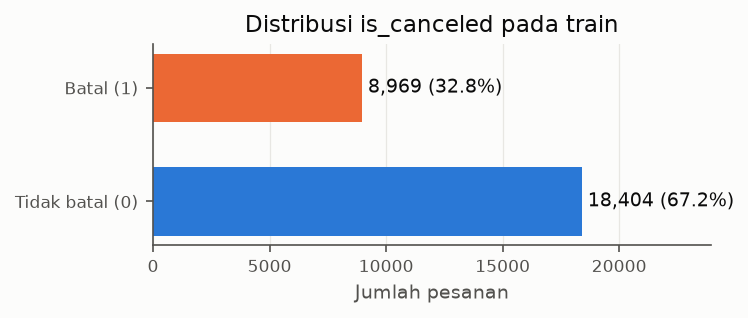
\includegraphics[width=0.6\textwidth]{target_distribution.png}
	\caption{Distribusi kelas target pada data latih}
	\label{fig:target-distribution}
\end{figure}
\endgroup
